\documentclass[a4paper,xcolor=table]{article}
%% Language and font encodings
\usepackage[english]{babel}
\usepackage[utf8x]{inputenc}
\usepackage[T1]{fontenc}

%% Sets page size and margins
\usepackage[a4paper,top=2.5cm,bottom=2cm,left=2.25cm,right=2.25cm,marginparwidth=2.25cm]{geometry}

%% Useful packages
\usepackage{amsmath}
\usepackage{graphicx}
%\usepackage[table,xcdraw]{xcolor}

%My Junk
\setlength{\footskip}{55pt}
\usepackage{fancyhdr}
\pagestyle{fancy}
\usepackage{textcomp}
\usepackage{gensymb}
\usepackage{hyperref}
\usepackage{readarray}
\usepackage{verbatimbox}
\usepackage{siunitx}

%All File Formatting
\setlength\parindent{0pt}

\usepackage{framed}
\usepackage[dvipsnames]{xcolor}
\usepackage{tcolorbox}
\usepackage{colortbl}
\usepackage{libertine} 
\usepackage{siunitx}
\usepackage{multirow}


%Special Section(s)
%\colorlet{shadecolor}{yellow}%FF3232}
\definecolor{safetyFrame}{HTML}{FFFFFF}
\newenvironment{safety}{%
\begin{tcolorbox}[width=\textwidth, colframe=safetyFrame, arc=1.5mm]
}%
{\end{tcolorbox}}


%Footer
\lfoot{
\includegraphics[height=1.5cm]{1000x350-Horiz-Logo-WhiteRed-BlackText.png}}

\title{The Long Weekend: Day 5 Review Analysis}
\author{Written by \textbf{Michael Uttmark}\\
		Checked by \textbf{-----}\\
        For the Stanford Student Space Initiative Biology Sub-team}

\newcommand{\tdt}{Terminal Deoxynucleotidyl Transferase}

%Custom Commands
\newcommand{\C}{\degree C}
\newcommand{\B}[1]{\textbf{#1}}
\newcommand{\stopPoint}{\begin{center}
\rule{0.5\textwidth}{.4pt}\\
\vspace{1mm} 
OPTIONAL STOP POINT\\
\rule{0.5\textwidth}{.4pt}
\end{center}}
\newcommand{\uL}{\micro{}L}



\newcommand{\Dilution}[4]{
\subsection{#2}
\begin{enumerate}
\item{Vortex #2 stock}
\item{Pipette #1\uL{} #2 into a PCR Tube}
\item{Pipette #3\uL{} #4 into solution}
\item{Vortex until mixed}
%\item{Pipette $#2\mu L$ Water into solution}
\end{enumerate}
}

%Well plate
\newcommand{\wellplate}[2]{
\getargsC{#1}
\begin{tabular}{*{1}{>{\columncolor{blue!20}}l}|l|l|l|l|l|l|l|l|l|l|l|l|}
\rowcolor{blue!20}%
 & 1  & 2  & 3  & 4  & 5  & 6 & 7 & 8 & 9 & 10 & 11 & 12\\ \hline
\ifdefined\argxii
A & \argi & \argii & \argiii & \argiv & \argv & \argvi & \argvii & \argviii & \argix & \argx & \argxi & \argxii \\ \hline\fi
\ifdefined\argxxiv
B & \argxiii & \argxiv & \argxv & \argxvi & \argxvii & \argxviii & \argxix & \argxx & \argxxi & \argxxii & \argxxiii & \argxxiv \\ \hline\fi
\ifdefined\argxxxvi
C & \argxxv & \argxxvi & \argxxvii & \argxxviii & \argxxix & \argxxx & \argxxxi & \argxxxii & \argxxxiii & \argxxxiv & \argxxxv & \argxxxvi \\ \hline\fi
\ifdefined\argxlviii
D & \argxxxvii & \argxxxviii & \argxxxix & \argxl & \argxli & \argxlii & \argxliii & \argxliv & \argxlv & \argxlvi & \argxlvii & \argxlviii \\ \hline\fi
\ifdefined\arglx
E & \argxlix & \argl & \argli & \arglii & \argliii & \argliv & \arglv & \arglvi & \arglvii & \arglviii & \arglix & \arglx \\ \hline\fi
\ifdefined\arglxxii
F & \arglxi & \arglxii & \arglxiii & \arglxiv & \arglxv & \arglxvi & \arglxvii & \arglxviii & \arglxix & \arglxx & \arglxxi & \arglxxii \\ \hline\fi
\ifdefined\arglxxxiv
G & \arglxxiii & \arglxxiv & \arglxxv & \arglxxvi & \arglxxvii & \arglxxviii & \arglxxix & \arglxxx & \arglxxxi & \arglxxxii & \arglxxxiii & \arglxxxiv \\ \hline\fi
\ifdefined\argxcvi
H & \arglxxxv & \arglxxxvi & \arglxxxvii & \arglxxxviii & \arglxxxix & \argxc & \argxci & \argxcii & \argxciii & \argxciv & \argxcv & \argxcvi \\ \hline\fi
\end{tabular}
}

\begin{document}

\maketitle

\section{Procedure Purpose}
To determine if reagents planned for use in a possible MVP (Minimally Viable Product) launch are viable after being left in solution for an extended period of time. 

\section{Overview}
The reagents will be removed from various storage temperatures (room temp ~23\C, ~-4\C\: and -20\C) and check for predicted florescence. They then will be combined with their “missing” components needed in order to preform a full \tdt{} homopolymer extension. At this point, 6\uL{} will be removed, heat denatured at 95\C, and stored at -20\C\: for future use. The samples will then be incubated and then heat denatured. The samples will then be examined via gel electrophoresis.\\

\section{Safety Information}
\begin{safety}
\begin{enumerate}
\item{\B{SYBR Green I} is a mutagen and can penetrate laboratory gloves in a relatively short period of time, please change your gloves in the event of contamination. See \url{http://www.sigmaaldrich.com/MSDS/MSDS/DisplayMSDSPage.do?country=US&language=en&productNumber=S9430&brand=SIAL} for more information on the specifics of SYBR Green I. 
}
\item{\B{Ethidium Bromide} is a \B{serious mutagen} and is \B{significantly carcinogenic}. If working with considerable amounts, a \B{fume hood and respirator} are warranted. For more information see \url{https://www.sciencelab.com/msds.php?msdsId=9927667}
}
\item{Working in a communal lab space is dangerous. Do not assume your fellow workers cleaned up sufficiently}
\end{enumerate}
\end{safety}
\section{Procedure}
\begin{enumerate}
\item{Remove the control samples from the room temperature, fridge and freezer storage.}
\item{Relabel samples if labels are no longer clear}
\item{Pipette samples into 96 well plate(s) in the order displayed below in Figure \ref{wellplate}.

\begin{figure}[ht]
\begin{center}
\wellplate{A1 H$_2$O A2 H$_2$O A3 H$_2$O . . . . . .
		   B1 H$_2$O B2 H$_2$O B3 H$_2$O . . . . . .
		   C1 H$_2$O C2 H$_2$O C3 H$_2$O . . . . . .
	   	   D1 H$_2$O D2 H$_2$O D3 H$_2$O . . . . . .
		   E1 H$_2$O E2 H$_2$O E3 H$_2$O . . . . . .
		   F1 H$_2$O F2 H$_2$O F3 H$_2$O . . . . . .
		   G1 J1     G2 J2     G3 J3 . . . . . .
		   H1 I1     H2 I2     H3 I3 . . . . . .}


\caption{96 Well Plate Sample Layout}
\label{wellplate}
 (1: Room Temp, 2: -4\C{}, 3: 20\C{})
\end{center}
\end{figure}
%\end{table}
}
\item{Run fluorescence tests using well plate viewer (Gain=50)}
\item{Pipette samples back into PCR tube}
\stopPoint
\item{Pipette the following reagents into PCR tubes as described in Figure \ref{table:instOne}}


\begin{figure}[ht]
\begin{center}\begin{tabular}{|l|l|l|l|l|l|l|l|l|}
\hline
        &TdT             & Sybr          & Primer 1        & Primer 2 & 5X TdT Buffer     & dTTPs & Water & Ethidium Bromide \\ \hline
A       & \texttimes{}              & \texttimes{}             & \texttimes{}               & \texttimes{}                 & \texttimes{}     & 1\uL{}   & 15.5\uL{}           & N/A \\ \hline
B       & \texttimes{}              & \texttimes{}             & 1.25\uL{}\,\textasteriskcentered{}  & 1.25\uL{}    {}\,\textasteriskcentered{} & \texttimes{}     & 1\uL{}   & 15.5\uL{}           & N/A \\ \hline
C       & \texttimes{}              & 1\uL{}\,\textasteriskcentered{}   & 1.25\uL{}\,\textasteriskcentered{}  & 1.25\uL{}    {}\,\textasteriskcentered{} & \texttimes{}     & 1\uL{}   & 15.5\uL{}           & N/A \\ \hline
D       & \texttimes{}              & 1\uL{}\,\textasteriskcentered{}   & 1.25\uL{}\,\textasteriskcentered{}  & 1.25\uL{}    {}\,\textasteriskcentered{} & \texttimes{}     & 1\uL{}   & 15.5\uL{}           & N/A \\ \hline
E       & 1\uL{}           & \texttimes{}             & 1.25\uL{}\,\textasteriskcentered{}  & 1.25\uL{}    {}\,\textasteriskcentered{} & 5\uL{}   & \texttimes{}     & 15.5\uL{}           & N/A \\ \hline
F       & 1\uL{}           & \texttimes{}             & \texttimes{}               & \texttimes{}                 & 5\uL{}   & \texttimes{}     & 15.5\uL{}           & N/A \\ \hline
G       & \texttimes{}              & \texttimes{}             & \texttimes{}               & \texttimes{}                 & \texttimes{}     & \texttimes{}     & 15.5\uL{}           & N/A \\ \hline
H       & \texttimes{}              & \texttimes{}             & \texttimes{}               & \texttimes{}                 & \texttimes{}     & \texttimes{}     & 15.5\uL{}           & N/A \\ \hline
I       & 1\uL{}           & 1\uL{}\,\textasteriskcentered{}   & 1.25\uL{}\,\textasteriskcentered{}  & 1.25\uL{}    {}\,\textasteriskcentered{} & 5\uL{}   & 1\uL{}   & \texttimes{}                & N/A \\ \hline
J       & 1\uL{}           & N/A           & 1.25\uL{}\,\textasteriskcentered{}  & 1.25\uL{}    {}\,\textasteriskcentered{} & 5\uL{}   & \texttimes{}     & 15.5\uL{}           & \texttimes{}   \\ \hline
\end{tabular}
\caption{Pipetting Instructions for PCR tubes}
\label{table:instOne}
\end{center}
Note: {}\,\textasteriskcentered{} indicates the need for a dilution from stock, “\B{\texttimes{}}” indicates a reagent already present. See following instructions for dilutions.

Note: The dNTPs were originally supposed to be dTTPs, but due to human error, they were not. This is reflected in Figure \ref{table:instOne}.
\end{figure}

\section*{Dilutions}
\Dilution{1}{SYBR Green I}{9}{Water}
\Dilution{2.5}{Primer 1}{22.5}{Water}
\Dilution{2.5}{Primer 2}{22.5}{Water}

\item{Incubate samples at 35\C{} for 60min}
\item{Stop the reaction by bringing the solution to 95\C{} for 10 minutes. }
\item{Then, bring to 2\C{} for 1 min for handling}
\stopPoint
\item{Pipette samples A-I from all groups into 96 well plate(s)}
\item{Run florescence tests using well plate viewer}
\stopPoint
\item{Prepare Agarose (Use Cobalt Chloride as a buffer for Gel)
\begin{enumerate}
    \item{To volume 80mL Buffer, add 2.2g Agarose (2.75\% Gel).}
    \item{Add 8\uL{} of SYBR Green to Agarose once lukewarm}
    \item{Refill Uytengsu Buffer stock}
    \end{enumerate}
}

\item{Prepare Primer Mix
\begin{enumerate}
    \item{Pipette 1\uL{} Primer 1 to PCR tube}
    \item{Pipette 1\uL{} Primer 2 to solution }
    \item{Pipette 78\uL{} Water to solution}
    \item{Vortex to Mix}
    \end{enumerate}
    }
\item{Plan Sample location in gels (see tables below)}
\item{Add Ladder to Gel  (1\uL{} of loaded solution)}
\item{Add samples and Primer Mix to gel (5\uL{} sample + 1\uL{} Loading dye $\Rightarrow$ 5\uL{} of loaded solution)}
\item{Run Gel at 100V for 20 minutes}
\item{Analyze Gel on Gel Viewer}
\item{Run Gel at 100V for 60 more minutes for a total of 80 minutes}
\item{Analyze Gel on Gel Viewer}
\item{Post pictures to SSI Slack}
\end{enumerate}
\section*{Stop Procedure}
\begin{enumerate}
\item{Pipette samples into PCR tubes if not already contained in an appropriate manner}
\item{Label containers}
\item{Freeze samples at -20\C{}}
\end{enumerate}

\begin{figure}[ht]
\addvbuffer[{0mm} \baselineskip]{\begin{tabular}{|l|l|l|l|l|}
\hline
Sample location, top to bottom (wells on the right)    & Gel 1 (Room Temp) & Gel 2 (-4\C{})	& Gel 3  (-20\C{}) & Gel 4 \\ \hline
1                                  & G2                & H1     		   & H3 			& J3 \\ \hline
2                                  & G1        		   & G3                & H2  			& J2 \\ \hline
3                                  & B3      		   & D3         	   & F3       		& J1*\\ \hline
4                                  & B2   	 		   & D2         	   & F2       		& I3 \\ \hline
5                                  & B1       		   & D1        	 	   & F1      		& I1 \\ \hline
6                                  & A3      		   & C3         	   & E3       		& I2 \\ \hline
7                                  & A2      		   & C2         	   & E2       		& \\ \hline
8                                  & A1      		   & C1        	       & E1       		& \\ \hline
9                                  & Primer    		   & Primer            & Primer   		& Primer \\ \hline
10                                 & Ladder  		   & Ladder     	   & Ladder   		& Ladder \\ \hline
\end{tabular}} \\ For a detailed description of the gels, see section \ref{sec:gelAnalysis}: Gels \& Accompanying Analysis.
\caption{Gel Table}
\label{tab:gelSampleArrangement}
\end{figure}

\section{Overall Analysis}

These data gathered by this experiment support the conclusion that the conditions present in samples A-C may result in the degradation of DNA over relatively short periods of time (\~13 days) at room temperature, -4\C{} and -20\C{}. However, the conditions in samples A-C still seem to be conducive to \tdt{} and it's continued activity after short periods of time at room temperature, -4\C{} and -20\C{}. Further, there seems to be evidence that, while the results from samples D, F and G are faint (in all strata), the conditions present in samples D, F and G seem to be conducive to \tdt{} and it's continued activity after short periods of time at room temperature, -4\C{} and -20\C{}. Nothing can be said about samples E and H from any of the gels. Further, these data support the hypothesis that \tdt{} works better when stored at -20\C{} rather than -4\C{} and better at -4\C{} than at room temperature (this relation is transitive). However, the quality control samples (the Is) indicate that there was a measurable amount of contamination from some source, probably human error. As such, while the results from A-C still seem to be indicative of truth (due to their strong signal and consistent trends), results derived from samples D, F and G are reasonably considered to be questionable and will need further verification in the future if their implications become paramount.

\section{Florescence Analysis}

\begin{figure}[ht]
\centering
\begin{tabular}{|l|l|l|l|l|l|l|l|l|l|}
\hline
    \quad{} &Sample                                                  & Room Temp. & -4\C{}  & -20\C{} & Deviation& $\lfloor 10^{-2}\rfloor$ &Room Temp. & -4\C{} & -20\C{}    \\ \hline
\cellcolor[HTML]{32CB00}                                              & A         & 5.07    & -1.41   & -2.77                       & 4.19                                                        &          & 0      & 0       & 0  \\ \cline{2-10} 
\cellcolor[HTML]{32CB00}                                              & F         & 1657.87 & 1657.87 & 28                          & N/A                                                         &          & 16     & 16      & 0  \\ \cline{2-10} 
\cellcolor[HTML]{32CB00}                                              & G         & 1657.87 & 1657.87 & 529.48                      & N/A                                                         &          & 16     & 16      & 5  \\ \cline{2-10} 
\multirow{-4}{*}{\cellcolor[HTML]{32CB00}} & H         & 1657.87 & 1657.87 & 1657.87                     & N/A                                                         &          & 16     & 16      & 17 \\ \hline
\cellcolor[HTML]{FFCB2F}       & J         & 1.98    & 37.22   & -0.72                       & 21.17                                                       &          & 0      & 0       & 0  \\ \hline
\cellcolor[HTML]{FE0000}                                              & B         & 2.81    & -2.8    & -3.7                        & 3.52                                                        &          & 0      & 0       & 0  \\ \cline{2-10} 
\cellcolor[HTML]{FE0000}                                              & C         & 83.16   & 39.46   & 9.05                        & 37.25                                                       &         & 0      & 0       & 0  \\ \cline{2-10} 
\cellcolor[HTML]{FE0000}                                              & D         & 145.85  & 18.46   & 2.83                        & 78.45                                                       &          & 1      & 0       & 0  \\ \cline{2-10} 
\cellcolor[HTML]{FE0000}                                              & E         & 771.85  & 340.93  & 18.18                       & 378.13                                                      &          & 7      & 3       & 0  \\ \cline{2-10} 
\multirow{-5}{*}{\cellcolor[HTML]{FE0000}}   & I         & 2.68    & 2.39    & 1.47                        & 0.63                                                        &          & 0      & 0       & 0  \\ \hline
\end{tabular}
\caption[Aggregated data pertaining to the florescence of samples.]{Aggregated data pertaining to the florescence of samples (see Section\ref{ssec:etbrAssay} for more information). Overflows replaced with 1657.87, the highest recorded value.}
\label{my-label}
\end{figure}

\subsection{SYBR Green I Related Sample Analysis}
Samples A, F, G and H were all expected to fluoresce when excited with \SI{485}{\nano\m} light (close to \SI{497}{\nano\m}, which is SYBR Green I's peak absorbance frequency for fluorescence \cite{sybrGreenI}).  These samples were expected to fluoresce because they contained SYBR Green I and at least one Primer. Some samples (B and E) contained SYBR Green I or a Primer, but not both, and were therefore not expected to fluoresce. Accordingly, samples F, G and H fluoresced significantly at Room Temperature, with their fluorescence tapering off from Room Temperature to -4\C{} and from -4\C{} to -20\C{}. This indicates that the change in temperature is positively correlated with the fluorescence of SYBR Green I in each samples respective storage conditions. However, it is important to note that F1, F2, G1, G2, H1 and H2 all overflowed. This missing data might contradict this observed trend. More data is needed for strong support to be established. As this data stands, little can be said for sure. 

Further, sample A did not fluoresce at all, and had a fluorescence pattern statistically identical to that of water. Either the sample was prepared incorrectly or this sample points to a severe instability of SYBR Green I in sample A's conditions. More data is needed for strong indication to be established and as this data stands, little can be said with any conviction. Still, this indicates that another experiment pertaining to A's conditions may be meritorious to complete. You can see this trend in Figure \ref{sybrTrend}.

\begin{figure}[ht]
\centering
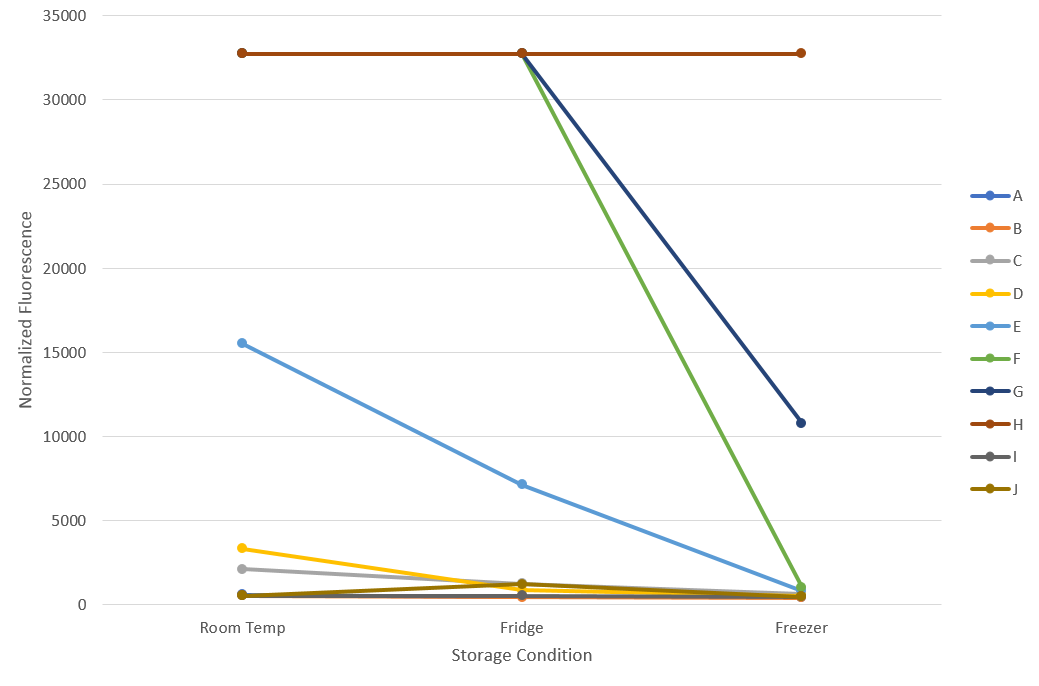
\includegraphics[width=.6\textwidth]{sybrTrend.png}
\caption{Storage Temperature \textit{vs.} Normalized Arbitrary Florescence Units}
\label{sybrTrend}
\end{figure}

Additionally, sample E fluoresced significantly even though it was supposed to contain DNA. This indicates one of two things: (1) there was an issue with contamination or (2) the instability of SYBR Green I caused this peculiar behavior. With the data at hand, it seems much more likely that there was an issue with contamination instead of an odd facet of SYBR Green's instability marvelously producing this behavior. With only three data points, little can be said for sure. D's measured florescence was insignificant at 1\%.

\subsection{Ethidium Bromide Related Sample Analysis}

The data in Figures \ref{etbr1} and \ref{etbr2} indicates that only J2 had active Ethidium Bromide. Moreover, only J2 fluoresced significantly when exposed to \SI{485}{\nano\m} light during the SYBR Green I assays. There are multiple things that could explain this, but most fall flat:
\begin{enumerate}
\item{Human Error: We did not add Ethidium Bromide to J1 or J3. This seems unlikely, as Ethidium Bromide has a very saturated color in solution, making it hard to pass over.}
\item{Ethidium Bromide degraded over time due to the temperature. This is unlikely, as J1 and J3 are the samples that didn't fluoresce, which implies that temperature isn't a particularly good predictor of fluoresce (however, one must always remember the imperative difference between correlation and causation).}
\item{The conditions of Ethidium Bromide caused degradation over time. This is also unlikely, as all three contained the same reagents.}
\item{Due to a human error, some reagent that was added to J2 was not added to J1 and/or J3 resulting in J2's anomalous behavior. This conclusion seems most likely, but more work should be done to support this hypothesis beyond our current data set with a cardinality of three.}
\end{enumerate}
\subsubsection{Ethidium Bromide Sample Assay}
\label{ssec:etbrAssay}
Regrettably, after the procedure was completed and samples disposed of, it was discovered that the Ethidium Bromide samples were examined via absorbance, not florescence. Moreover, the samples were examined at \SI{258}{\nano\m} rather than \SI{360}{\nano\m} which is the peak absorbency frequency for Ethidium Bromide \cite{etbrSpec}. However, as we can see from Figure \ref{fig:etbrAbs}, there is still a significant absorbance of light at \SI{258}{\nano\m} (roughly 40\%). As such, we can still determine that the Ethidium Bromide should still be detectable via absorption data. Moreover, it's important to note that the solvent (water) does not have a significant absorbance at \SI{258}{\nano\m} \cite{uvWaterAbs} and therefore should not impact our results significantly (See Figure \ref{fig:waterAbs}).

\begin{figure}[ht]
\begin{center}
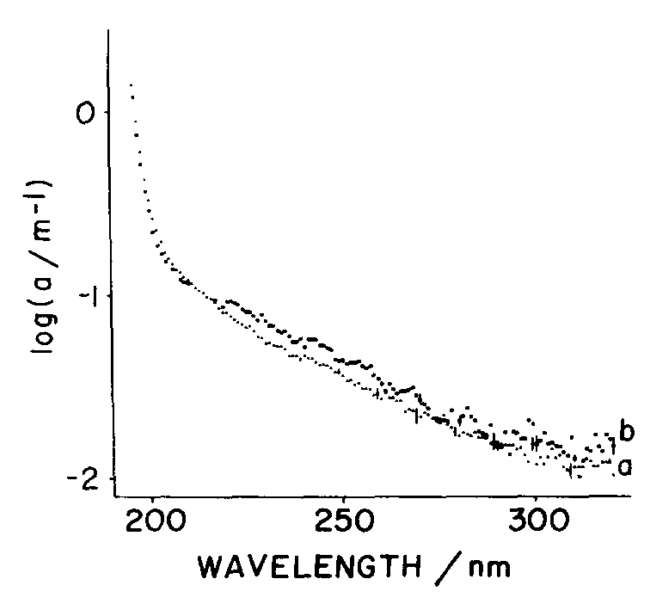
\includegraphics[width=.33\textwidth]{waterAbsProf.png}
\caption{Measured ultraviolet absorption spectra of liquid water\cite{uvWaterAbs}}
\label{fig:waterAbs}
\end{center}
\end{figure}

\begin{figure}[ht]
\begin{center}
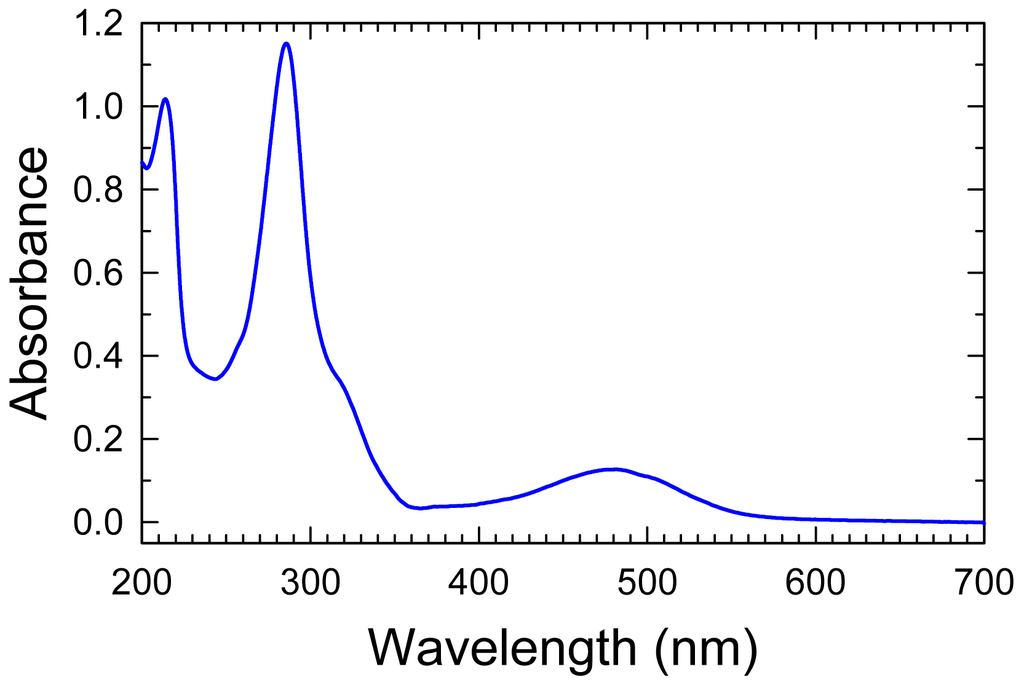
\includegraphics[width=.33\textwidth]{etbrAbs.png}
%Attribution
\caption{Absorption spectrum of Ethidium Bromide in water at room temperature}
{\small Image by Mark Somoza (Own work) [\href{http://www.gnu.org/copyleft/fdl.html}{GFDL}, \href{http://creativecommons.org/licenses/by-sa/3.0/}{CC-BY-SA-3.0} or \href{http://creativecommons.org/licenses/by/2.5}{CC BY 2.5}], via Wikimedia Commons}
\label{fig:etbrAbs}
\end{center}
\end{figure}




\section{Gels \& Accompanying Analysis}
\label{sec:gelAnalysis}
Continued on next page.

\newcommand{\gel}[3]{
\begin{figure}[ht]
\label{#3}
\begin{center}
\includegraphics[width=0.9\textwidth]{#1}
\caption{#2}
\end{center}
\subsection{#2 Analysis}
#3 (More images of this gel below.)
\end{figure}
}

\newcommand{\gels}[4]{
\begin{figure}[ht]
\label{#3}
\begin{center}
\includegraphics[width=0.9\textwidth]{#1}\\
\includegraphics[width=0.9\textwidth]{#2}
\caption{#3}
\end{center}
#4
\end{figure}
}



\gel{gels/tlw-1-day5-reading1-80min.png}{Gel 1}{
As one can clearly see above (or rather not see) samples A and B are not visible. Further, there is no residue in their wells (normal activity for most DNA samples). These two facts indicate that these samples either were not added to the gel or did not contain DNA. (It is extremely unlikely that SYBR I would have stained the other samples and excluded A and B). We see extension in sample G2, but not in G1. This indicates that G1 did not see extension at room temperature, even though it was had all the needed reagents except for water. Further, this provides evidence that storing a "full pot" of reagents at room temperature leads to inactive reagents after 5 days, which is a relatively short period of time. However, this also provides support for the conclusion that storage at -4 degrees Celsius rather than at room temperature can in fact make a difference in reagent performance.
}
\begin{comment}
\gels{gels/tlw-1-day5-reading1-20min.png}{gels/tlw-1-day5-reading1-80min__1_.png}{Gel 1}{The initial 20 minute reading on the left and the second 80 minute reading on the right.}

\gel{gels/tlw-2-day5-reading1-80min.png}{Gel 2}{anasdfjhalskdjfhalksdjfhalkjdfsdhalksjdfhalkjsdhf}

\gels{gels/tlw-2-day5-reading2-80min.png}{gels/tlw-2-day5-reading1-80min__1_.png}{Gel 2}{The initial 20 minute reading on the left and the second 80 minute reading on the right.}

\gel{gels/tlw-3-day5-reading1-80min.png}{Gel 3}{anasdfjhalskdjfhahlksdjfhalkjdfshalksjdfhalkjsdhf}

\gels{gels/tlw-3-day5-reading2-80min.png}{gels/tlw-3-day5-reading1-80min__1_.png}{Gel 3}{The initial 20 minute reading on the left and the second 80 minute reading on the right.}

\gel{gels/tlw-4-day5-reading1-80min.png}{Gel 4}{anasdfjhalskdjfhaalksdjfhalkjdfshalksjdfhalkjsdhf}

\gels{gels/tlw-4-day5-reading2-80min.png}{gels/tlw-4-day5-reading1-80min__1_.png}{Gel 4}{The initial 20 minute reading on the left and the second 80 minute reading on the right.}
\end{comment}

\begin{figure}[ht]
\begin{center}
\wellplate{585.5	554	459.5	484	433	440.5	417.5	447.5	430	449	454	448.5
541.5	545	432.5	449.5	415	434.5	428.5	411	438.5	433	442.5	459.5
2104.5	460.5	1254.5	445	663	429.5	434.5	409.5	435	421.5	454.5	450
3324	457	846	468	542	439.5	412	438.5	420.5	440	443	452
15500.5	461	7118.5	439	840.5	427	421.5	461.5	419.5	435	465.5	464.5
OVRFLW	509	OVRFLW	496.5	1031.5	451	435.5	441	425.5	435	477	451.5
OVRFLW	1.693	OVRFLW	3.724	10786	1.679	454	454	437	467.5	477	476
OVRFLW	539	OVRFLW	533.5	32735	515.5	462.5	458	467	468	493	464.5}

\label{tab:rawAvg}
\caption{Averages of the values from Figure \ref{read1} and Figure \ref{read2} with Ethidium Bromide sample related values (G2, G4 and G6) replaced with values from Figure \ref{etbr2}. Please note that the Ethidium Bromide related values are in different units, see Section \ref{ssec:etbrAssay} for more information.}
\end{center}
\end{figure}

\begin{figure}[ht]
\begin{center}
\wellplate{589	559	451	480	450	437	401	449	423	444	457	443
555	538	435	429	412	452	422	410	445	456	441	457
2123	480	1297	450	663	436	449	418	445	417	468	465
4665	471	799	469	548	427	417	417	421	430	450	450
15583	467	13244	429	1013	433	414	472	414	450	466	463
OVRFLW	499	OVRFLW	470	1053	443	420	444	416	420	472	437
OVRFLW	504	OVRFLW	1234	10934	490	453	449	439	464	478	463
OVRFLW	548	OVRFLW	536	34587	541	463	460	469	461	497	444
}

\caption{Read One: Excitation: \SI{485}{\nano\m},  Emission: \SI{528}{\nano\m} (SYBR Green I Fluorescence Assay)}
\label{read1}
\end{center}
\end{figure}


\begin{figure}[ht]
\begin{center}
\wellplate{582	549	468	488	416	444	434	446	437	454	451	454
528	552	430	470	418	417	435	412	432	410	444	462
2086	441	1212	440	663	423	420	401	425	426	441	435
1983	443	893	467	536	452	407	460	420	450	436	454
15418	455	993	449	668	421	429	451	425	420	465	466
OVRFLW	519	OVRFLW	523	1010	459	451	438	435	450	482	466
OVRFLW	547	OVRFLW	1188	10638	456	455	459	435	471	476	489
OVRFLW	530	OVRFLW	531	30883	490	462	456	465	475	489	485
}

\caption{Read Two: Excitation: \SI{485}{\nano\m},  Emission: \SI{528}{\nano\m} (SYBR Green I Fluorescence Assay)}
\label{read2}
\end{center}
\end{figure}

\begin{figure}[ht]
\begin{center}
\wellplate{1.72	1.706	1.661	1.698	1.666	1.661	1.693	1.697	1.706	1.75	1.763	1.773
1.681	1.653	1.661	1.661	1.625	1.647	1.632	1.642	1.663	1.696	1.723	1.753
1.754	1.682	1.686	1.662	1.621	1.644	1.655	1.654	1.729	1.709	1.716	1.744
1.721	1.663	1.641	1.635	1.623	1.618	1.633	1.626	1.646	1.678	1.714	1.746
2.015	1.67	1.667	1.636	1.617	1.61	1.625	1.649	1.68	1.689	1.761	1.78
1.997	1.757	1.953	1.721	1.68	1.685	1.68	1.705	1.736	1.749	1.799	1.832
2.702	1.693	2.218	3.709	1.669	1.678	1.691	1.696	1.724	1.739	1.771	1.829
1.895	1.809	2.726	1.839	1.801	1.722	1.719	1.762	1.782	1.767	1.858	1.881}

\caption{Read One: Absorbance at \SI{285}{\nano\m} (Ethidium Bromide Assay, see \ref{ssec:etbrAssay} for more information)}
\label{etbr1}
\end{center}
\end{figure}

\begin{figure}[ht]
\begin{center}
\wellplate{1.719	1.706	1.662	1.697	1.664	1.659	1.692	1.697	1.705	1.751	1.764	1.773
1.68	1.654	1.661	1.66	1.623	1.646	1.631	1.642	1.663	1.695	1.723	1.752
1.757	1.683	1.685	1.661	1.621	1.643	1.655	1.654	1.729	1.708	1.715	1.743
1.719	1.663	1.639	1.634	1.622	1.618	1.633	1.628	1.649	1.679	1.714	1.745
2.016	1.669	1.667	1.636	1.616	1.609	1.626	1.649	1.68	1.688	1.76	1.78
1.987	1.757	1.939	1.721	1.68	1.686	1.681	1.707	1.734	1.749	1.801	1.833
2.667	1.693	2.129	3.724	1.668	1.679	1.691	1.697	1.723	1.738	1.771	1.831
1.879	1.808	2.613	1.841	1.793	1.722	1.72	1.763	1.781	1.768	1.858	1.882}

\caption{Read Two: Absorbance at \SI{285}{\nano\m} (Ethidium Bromide Assay, see \ref{ssec:etbrAssay} for more information)}
\label{etbr2}
\end{center}
\end{figure}

\bibliographystyle{ieeetr}
\bibliography{SSI-Synthesis}
\end{document}